\section{An\'alisis}

\subsection{Descripci\'on}

Este prototipo se encarga de la clasificaci\'on de conversaciones en peligrosas o no peligrosas de acuerdo al Nivel 5.

\subsection{Objetivo}
Formular un modelo matem\'atico que permitir\'a la clasificaci\'on de conversaciones peligrosas o no peligrosas de acuerdo al nivel 5 de la matriz de caracterizaci\'on de comportameniento.

\subsection{Caracter\'isticas}
\begin{description}
\item[FEAT1] Plantear el clasificador mediante un modelo matem\'atico usando regresi\'on log\'istica.
\item[FEAT2] Entrenar el clasificador con conversaciones etiquetadas como peligrosas.
\item[FEAT3] Entrenar el clasificador con conversaciones etiquetadas como no peligrosas.
\item[FEAT3] Verificar la eficiencia del clasificador mediante una matriz de confusi\'on.
\end{description}			

\subsection{Restricciones}

\begin{itemize}
\item Clasificador entrenado con aprendizaje supervisado.
\item Implementaci\'on de clasificador en Octave 3.8
\end{itemize}


\subsection{Marco Te\'orico}
\subsubsection{Algoritmo de regresi\'on log\'istica}

El algoritmo de regresi\'on logistica es un m\'etodo estad\'istico que es usado para determinar la ocurrencia de un evento simple valorando diferentes factores.  

Este m\'etodo es adecuado cuando la variable o vector de respuesta $Y$ admite varias categor\'ias de respuesta, es decir, es polit\'omica. Pero es de mayor utilidad cuando \'unicamente nos encontramos con dos posibles respuestas.

Dicho lo anterior, podemos deducir que la variable dependiente $y$ tomar\'a el valor 1 si ocurre el suceso, y por el contrario el valor 0 si no ocurre. La ecuaci\'on \ref{eq:vectory} muestra del conjunto de posibles valores de un clasificador de 2 clases.
\begin{equation}\label{eq:vectory}
y \in {0,1}
\end{equation}

El objetivo de este algortimo es diese\~nar un m\'odelo basado en la formumlaci\'on de una funci\'on $h_{\theta}(x)$ de tal forma que:

\begin{equation}\label{eq:funcionHipotesis}
0 \leq h_{\theta}(x) \leq 1
\end{equation}

La ecuaci\'on \ref{eq:funcionHipotesis} estada dada bajo una relaci\'on de compocici\'on cuyo dominio independiente es el producto matricial del vector de entrada $x$ con un vector de param\'etros $\theta$. La ecucio\'on \ref{eq:composicion}

\begin{equation}\label{eq:composicion}
h_{\theta}(x) = g(\theta x)
\end{equation}

La funci\'on $g(z)$ est\'a descrita en relaci\'on a la funci\'on sigmoide descrita en la ecuaci\'on \ref{eq:sigmoide} la cual es utilizada como curva de aprendizaje de sistemas complejos.


\begin{equation}\label{eq:sigmoide}
g(z) = \frac{1}{1+e^z}
\end{equation}
donde:
\begin{equation}
z = \theta_{0}x_{0}+ \theta_{1}x_{1} + ... +  \theta_{n}x_{n}
\end{equation}

La figura \ref{fig:sigmoide} muestra la gr\'afica de la funci\'on sigmoide cuyo comportamiento est\'a dado por las ecuaciones \ref{eq:limite1} y \ref{eq:limite2}

\begin{equation}\label{eq:limite1}
\lim_{z \to \infty} g(z) = 1
\end{equation}

\begin{equation}\label{eq:limite2}
\lim_{z \to -\infty} g(z) = 1
\end{equation}
donde:
\begin{equation}
z = \theta_{0}x_{0}+ \theta_{1}x_{1} + ... +  \theta_{n}x_{n}
\end{equation}

\begin{figure}[h]
	\begin{center}
		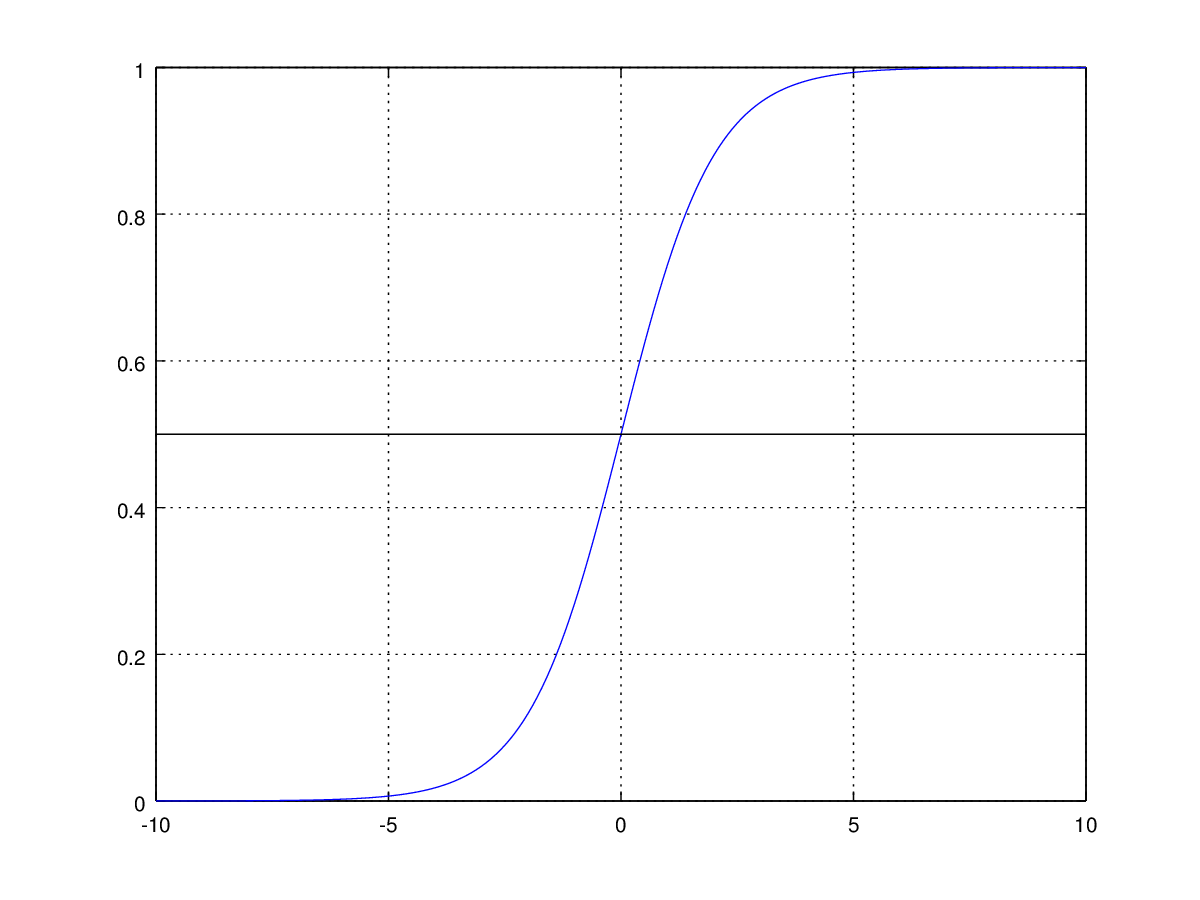
\includegraphics[scale=.5]{images/sigmoide}
		\caption{Gr\'afica de la funci\'on sigmoide}
		\label{fig:sigmoide}
	\end{center}
\end{figure}

La manera en que se interpreta el resultado de la funci\'on sinoide es la siguiente.

Sea $x$ un vector donde cada componente indica una caracter\'istica en particular:

\begin{equation}
x  = 
\begin{bmatrix}
x_{0} \\
x_{1} \\
\vdots \\
x_{n}
\end{bmatrix}
\end{equation}

Entonces si $h_{\theta}(x) = 0.7$ decimos que hay un 70\% de probabilidad de que el vector $x$ pertenezca a la clase etiquetada con valor 1.

Dentro de este algoritmo podemos definir una frontera de desici\'on la cual indique el umbral de valores para que un vector pertenezca a una clase u otra.

Por ejemplo $y = 1$ si se cumple la condici\'on: 
\begin{equation}
h_{\theta}(x) \geq 0.5
\end{equation}
De lo contrario $y = 0$ si
\begin{equation}
h_{\theta}(x) < 0.5
\end{equation}

El objetivo del algoritmo es encontrar el vector $\theta$ \'optimo de tal manera de formular un m\'odelo lineal que separe las clases como el ejemplo de la figura \ref{fig:ejemploClases}

\begin{figure}[h!]
	\begin{center}
	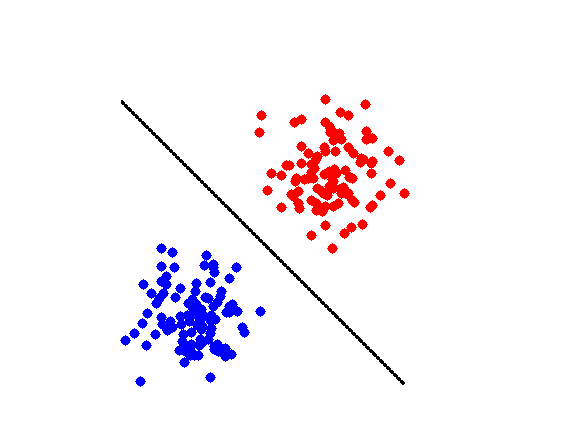
\includegraphics[scale=.3]{images/clasesejemplo}
	\caption{Ejemplo de separaci\'on de Clases}
	\label{fig:ejemploClases}
	\end{center}
\end{figure}

Para evaluar el costo de los parametros del vector $\theta$ se tiene la siguiente ecuaci\'on:
\begin{equation}
costo(h_{\theta}(x),y) = -yln(h_{\theta}(x))-(1-y)ln(1-h_{\theta}(x))
\end{equation}

\section{Dise\~no}
\subsection{Arquitectura}
La figura \ref{fig:arquitecturaClasificador} muestra la arquitectura del prototipo de clasificaci\'on del Nivel 5.
\begin{figure}[h]
	\begin{center}
	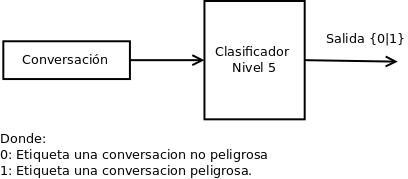
\includegraphics[scale=.5]{images/arquitecturaClasificador}
	\caption{Ejemplo de separaci\'on de Clases}
	\label{fig:arquitecturaClasificador}
	\end{center}
\end{figure}

\section{Pruebas}

\subsection{Entrenamiento con 3 variables}
Se realiz\'o el entrenamiento con 3 variables las cuales corresponden a las componentes del vector generado por el prototipo 1 con la siguiente lista de palabras:
\begin{itemize}
\item Pene
\item Vagina
\item Desnudo
\end{itemize}

Estas variables generaron un vector $\theta$ con los siguientes valores:

\begin{equation}
\theta = 
\begin{bmatrix}

-0.613684 \\
 0.904610 \\
 1.221655 \\
 0.726040
\end{bmatrix}
\end{equation}

La tabla \ref{tab:confucion1} muestra la tabla de confusi\'on de este entrenamiento.


\begin{table}[h]
\begin{center}
\begin{tabular}{c|c|c|c|c|}
\multicolumn{5}{c}{Predicci\'on} \\
\cline{2-5}
& & Conversaci\'on No Peligrosas & Conversaci\'on Peligrosas &  Presici\'on \\
\cline{2-5}
\multirow{2}{*}{Actual} & Conversaci\'on no Peligrosa & 17 & 3 & 85\% \\
\cline{2-5}
& Conversaci\'on Peligrosa &  6 & 33 & 84\% \\
\cline{2-5}

\end{tabular}
\caption{Tabla de Confuci\'on con 3 rasgos}
\label{tab:confucion1}
\end{center}
\end{table}

Con esto se tiene una precisi\'on de un 84.5\% del clasificador.
La figura \ref{fig:separabilidad} muestra de manera gr\'afica un plano que muestra la separabilidad de las clases con vectores de 3 componentes.

\begin{figure}
	\begin{center}
	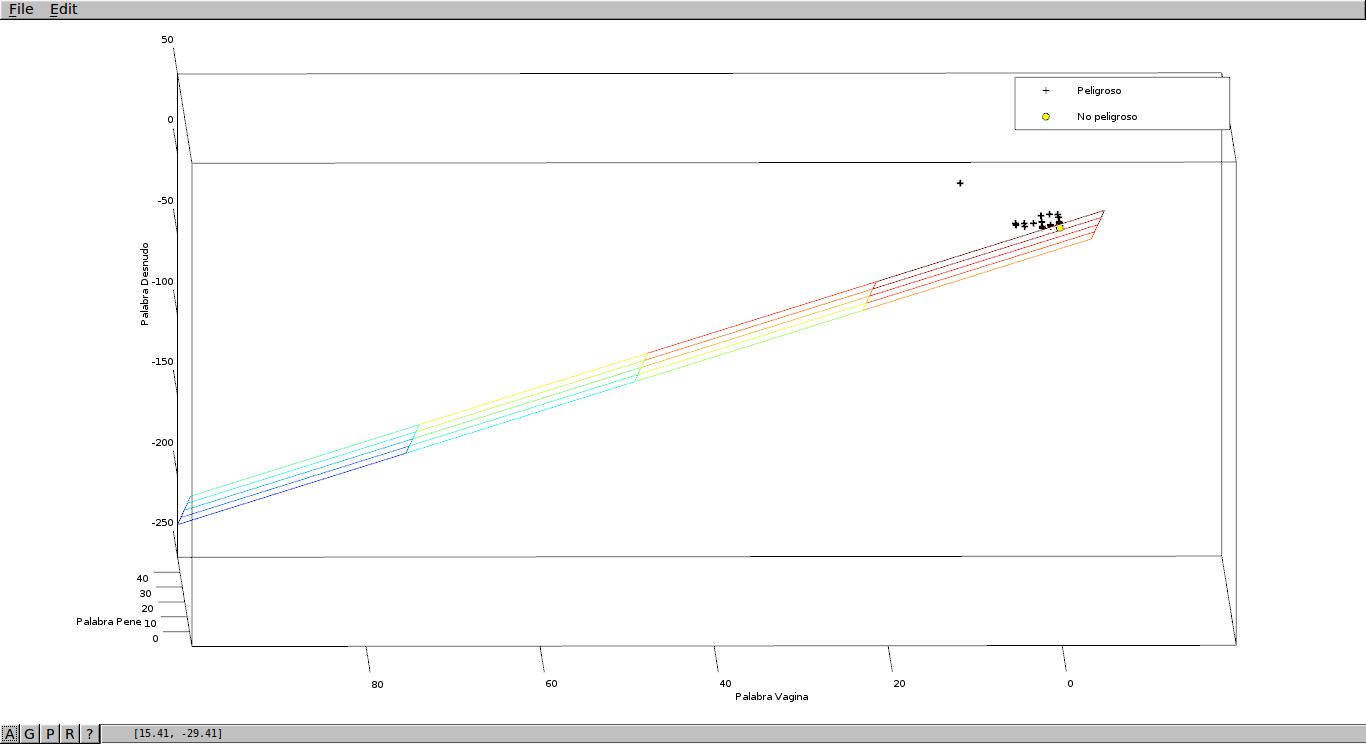
\includegraphics[scale=.4]{images/separavilidad}
	\caption{Gr\'afica que muestra la separabilidad del clasificador.}
	\label{fig:separabilidad}
	\end{center}
\end{figure}


\subsection{Entrenamiento con 14 variables}
Se realiz\'o el entrenamiento con 3 variables las cuales corresponden a las componentes del vector generado por el prototipo 1 con la siguiente lista de palabras:
\begin{itemize}
\item chupar 
\item coger
\item follar
\item lamer
\item besar
\item pene 
\item vagina
\item masturbar
\item sexo
\item pechos
\item tetas
\item clitoris
\item tragar
\item violar
\end{itemize}

Estas variables generaron un vector $\theta$ con los siguientes valores:

\begin{equation}
\theta = 
\begin{bmatrix}

-1.027760 \\
 0.704011 \\
 0.907893 \\
 0.588279 \\
 0.529208 \\
 0.203309 \\
 0.104863 \\
 1.167757 \\
 0.975621 \\
 0.348992 \\
 0.541306 \\
 0.622848 \\
 0.233392 \\
 0.039713 \\
 -0.066605
 
\end{bmatrix}
\end{equation}

La tabla \ref{tab:confucion2} muestra la tabla de confusi\'on de este entrenamiento.


\begin{table}[h]
\begin{center}
\begin{tabular}{c|c|c|c|c|}
\multicolumn{5}{c}{Predicci\'on} \\
\cline{2-5}
& & Conversaci\'on No Peligrosas & Conversaci\'on Peligrosas &  Presici\'on \\
\cline{2-5}
\multirow{2}{*}{Actual} & Conversaci\'on no Peligrosa & 20 & 0 & 100\% \\
\cline{2-5}
& Conversaci\'on Peligrosa &  2 & 41 & 95\% \\
\cline{2-5}

\end{tabular}
\caption{Tabla de Confusi\'on con 3 rasgos}
\label{tab:confucion2}
\end{center}
\end{table}

Con esto se tiene una precisi\'on de un 96.72\% del clasificador.


Para el valor de prediction tenemos 

%\begin{equation}
%\frac{TruePositives}{TruePositiveP + FalseNegatives)

\begin{equation}\label{eq:sigmoide}
\frac{TruePositives}{TruePositive + FalsePositives} = \frac{41}{41+2} = 0.9534
\end{equation} 

El valor del recall es: 

\begin{equation}\label{eq:sigmoide}
\frac{TruePositives}{TruePositive + FalseNegatives} = \frac{41}{41+2
0} = 1
\end{equation}

Ambos valores nos indican que esa cantidad de desciriptores del clasificador lo hacen tener un buen desempe\~no.


